\documentclass[12pt]{article}

\usepackage{graphicx}
\usepackage{tikz}
\usepackage{array}

\title{AMath Tea Time --- Puzzle \#11}
\author{}
\date{\vspace{-1cm}13 October 2015}

\begin{document}

\maketitle
\pagenumbering{gobble}

\subsection*{Problem}

\noindent {\bf Problem \#1:} I have seven of each of the seven types of
tetrominoes below. Can I arrange them to make a $28 \times 7$ rectangle? \\

\noindent {\bf Problem \#2:} Using only the first tetromino in the second row,
what is the maximum number of this tetromino that you can place on an $8 \times
8$ board without overlapping? (This piece is called the {\it S}, {\it inverse
  skew}, or {\it right snake} tetromino.) What about using only the second
tetromino in the second row? (This piece is called the {\it T} or {\it tetris}
tetromino.)

\begin{figure}[h]
  \centering
  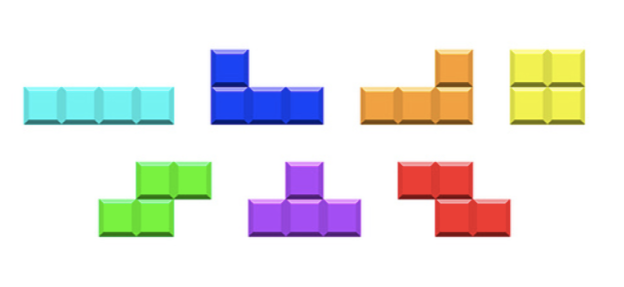
\includegraphics[width=.75\textwidth]{tetromino.png}
\end{figure}

\subsection*{Hints}

{
\par\vspace*{\fill}
\noindent \small \it
If you have any puzzles to share then send them my way at {\tt
  cswiercz@uw.edu}!
}

\end{document}
